% Template for ICME 2018 paper; to be used with:
%          spconf.sty  - ICASSP/ICIP/ICME LaTeX style file, and
%          IEEEbib.bst - IEEE bibliography style file.
% --------------------------------------------------------------------------
\documentclass{article}
\usepackage{spconf,amsmath,epsfig}
\usepackage{graphicx}
\usepackage{subfigure}
\pagestyle{empty}
\usepackage{epstopdf}
\usepackage{color}


\definecolor{red}{rgb}{1.0,0.0,0.0}
\definecolor{blue}{rgb}{0.0,0.0,1.0}
\definecolor{purple}{rgb}{0.5,0.0,0.5}


\newcommand{\comments}[1]{}
\newcommand{\xj}[1]{\textcolor{red}{(xuejin:#1)}}
\newcommand{\md}[1]{\textcolor{blue}{#1}}
\newcommand{\camin} {\mathbf{K}}
\newcommand{\camex}{\mathbf{M}}
\newcommand{\vb}[1]{\mathbf{#1}}



\begin{document}\sloppy

% Example definitions.
% --------------------
\def\x{{\mathbf x}}
\def\L{{\cal L}}


% Title.
% ------
\title{A Hybrid System Integrating Calibration and Registration for Accurate 3D Reconstruction}
%
% Single address.
% ---------------
\name{Paper 1375}
\address{ }



\maketitle


%
\begin{abstract}
With the development of virtual and augmented reality, 3D reconstruction for indoor scenes based on multi-camera systems has become increasingly popular recently.
%
The quality of 3D reconstructions relies on many factors, including the multi-view camera calibration accuracy and the depth estimation quality in each single view.
%
In this paper, we propose a hybrid system which integrates the global camera parameter estimation and  3D model registration instead of traditional pairwise frameworks, to produce high quality 3D models.
%replace the traditional pairwise relations of both camera and model fusion to a global framework.
%
First, a global bundle adjustment is adopted to increase the accuracy of camera pose estimation.
%We use checkerboard corners to optimize the camera extrinsic parameters globally which are obtained by pairwise camera calibration methods.
Second, a point cloud registration is used to fuse the inaccurate depth maps to a 3D model.
We use the Iterative Closest Point (ICP) algorithm to register the point clouds estimated from different views to minimize the model deviation.
The experimental results show the promising effect of our method to produce high-quality models.
\end{abstract}
%
\begin{keywords}
Multi-camera system, 3D reconstruction, camera calibration, point cloud registration
\end{keywords}
%

\section{Introduction}

Real-time indoor 3D reconstruction from multiple views has become more and more prevalent in recent years~\cite{dou2016fusion4d,orts2016holoportation}. Multi-camera systems using RGBD cameras have many advantages such as a wider horizon compared with the systems based on a single camera, and are widely used in many kinds of applications. However, both the intrinsic and extrinsic parameters of the multi-camera systems are required to be calibrated accurately in order to achieve a high-quality and real-time 3D reconstruction of an entire object, such as a person or a furniture object.

For a single camera system, the accurate intrinsic parameters can be achieved by many internal calibration methods or toolboxes~\cite{zhang2000flexible,zhang2004camera}. Many efficient methods have also been developed for the calibration of different types of multi-camera calibration. 
%
One widely proposed approach for the multi-camera calibration is to use special calibration objects, such as patterns, rig or similar. 
Li et al. proposed a toolbox to calibrate the system which uses a feature descriptor based calibration pattern~\cite{Li2013A}. 
\xj{...confusing here}
%
The pattern can be automatically detected even if the pattern is partially visible in an image. The toolbox yields good results especially on the systems with a few cameras (three or four) with minimal overlapping fields of view. 
\xj{what do you mean by minimal?}
%
Zhao and Liu proposed an algorithm based on 1D objects \xj{what do you mean by 1D?} which works well on a triple camera system~\cite{zhao2008practical}. The algorithm integrates a rank-4 factorization with the standard 1D camera calibration method and is much more convenient than plane-based algorithms. 
Svoboda et al. gives a method that only requires a bright-spot object like a laser pointer~\cite{svoboda2005convenient}. Waving the object which can be easily detected in each image through the working space is the only work requested. 
\xj{Authors: A and B or A et al. Modify all the reference in the draft. }
Kalibr~\cite{Maye2013Self} is a free toolbox that solves the multiple camera calibration problems. 
%
It could produce a good estimate but requires that neighboring cameras have overlapping fields of view. 
However, if the system contains many cameras and they do not share the same overlapping fields of view, the calibration process should be simply repeated for each pair of cameras.
\xj{So any problem of the Kalibr?}

Another kind of methods which is commonly used is self-calibration. These methods do the calibration using the constraints and correspondences from the images without any special calibration objects. 
Bundler~\cite{snavely2006photo} is a structure-from-motion toolbox using the unordered images captured from different views. The pose of all cameras can be estimated simultaneously with the 3D point positions. 
It uses SIFT keypoint detector~\cite{lowe2004distinctive} which works well on outdoor scenes but weak on indoor cases because of the lack of rich textures. Vasconcelos~\cite{vasconcelos2012minimal} proposed a solution to calibrate a camera with two other calibrated cameras using independent pairwise point correspondences.
% 
Bushnevskiy~\cite{bushnevskiy2016multicamera} presented a novel approach for the estimation of the geometry of the multi-camera system. The algorithm enforces constraints arising from the visible epipoles and is especially suitable for dome-like indoor cases.

All these methods use RGB images to calibrate the multi-camera system and achieve good results. However, not only RGB cameras, other kinds of sensors are also widely used in 3D reconstruction system nowadays, like Near Infra-Red (NIR) cameras. If there are such cameras within the system used to estimate the depth, the error of the final result of the 3D reconstruction not only comes from the calibration of the RGB cameras but also from the depth estimation. Many research have been done on the depth estimation~\cite{scharstein,Bleyer2011PatchMatch}, whereas the error can not be eliminated entirely. How to minimize the error of the whole reconstruction to achieve an accurate model is a problem.

In this paper, we present an efficient algorithm to optimize the extrinsic camera parameters for indoor 3D reconstruction. To avoid from accumulative error caused by the repetitive calibration for each pair of cameras, we use a global camera calibration method and optimize all the camera parameters consistently. Furthermore, we use the point cloud registration method to adjust the result of the reconstruction. This can effectively decrease the error result from the depth estimation and obtain a high-quality 3D reconstruction.



\section{overview}
\label{sec:overview}

\xj{I add the problem definition here.}


%\textbf{Problem Definition.}
A multi-camera system is set up to capture objects in an indoor scene, as shown in Fig.~\ref{fig:rig}.
%The cameras in our 3D reconstruction system are placed on the periphery of the room pointing inwards, only the neighboring cameras have overlapping fields of view. \xj{what is the point of this overlapping fov?}
%
$K$ ($K=8$) camera pods are installed around the working space looking inwards for a full capture.
Each camera pod consists of one color camera and two Near Infra-Red cameras. A laser pointer is used to produce special patterns. From the pair of images of the projected patterns captured by the two NIR cameras, a depth map $D_k$ can be estimated using PatchMatch stereo algorithm~\cite{Bleyer2011PatchMatch}.
There are also several alternative depth cameras or depth estimation algorithm to obtain the depth map of each view. Most of them produce a rough depth map with noise and errors, as Fig.~\ref{fig:depthmap} shows.
How to improve the quality of depth map is beyond the scope of this paper.

\begin{figure}
	\centering
	\includegraphics[width=\columnwidth]{image/rig.jpg}
	\caption{Our multi-camera system with 8 camera pods pointing inwards.}
	\label{fig:rig}
\end{figure}


%
Under the assumption of pinhole camera, each camera has a group of parameters including the intrinsic matrix $K$ and extrinsic matrix $M$ to project a point $P$ in the 3D space to its image plane as
\begin{equation}\label{eq:cam-proj}
z_{p}\mathbf{x}=\mathbf{K}\mathbf{M}\mathbf{p},
\end{equation}
where $\mathbf{p}=(x,y,z,1)^{T}$ is the homogeneous coordinate of $P$, and $\mathbf{x}=(u,v,1)^{T}$ is the homogeneous coordinate of its projected point on the image plane.
%

From the depth map estimated by each camera pod, a partial point cloud can be reconstructed by back-projecting each pixel in the depth map into the 3D space according to the pose parameters of each camera.
%
A 3D model can be obtained by fusing the $K$ point clouds.
%
%
Ideally, with accurate depth $z_p$ of each image point $\vb{x}$, and accurate camera parameters $\camin$ and $\camex$, the image pixels captured in different views can be back-projected to the 3D space and well aligned to a 3D point $\vb{p}$.
To reconstruct a high-quality model, our algorithm consists of two main parts.
%
The first part is a global camera calibration method to estimate the camera parameters $\{\camin_k, \camex_k\}^{K}_{k=1}$ as accurate as possible, as described in Sec.~\ref{sec:global-calib}.
The second is a registration method to produce 3D point clouds as consistent as possible from in-accurate depth $z_p$, as described in Sec.~\ref{sec:registration}.
\xj{Explain with a pipeline figure.}
\md{To Do}


\comments{

Our algorithm consists of two main parts. Firstly, we use the toolbox Kalibr~\cite{Maye2013Self} to calibrate our multi-camera system and achieve the intrinsic and initial extrinsic parameters of all our cameras. Then we use a checkerboard as the calibration object, detect the corners on it and do the global extrinsic parameters optimization, as described in Sec.~\ref{sec:global-calib}.
%
Secondly, we use the camera parameters and the input RGB and depth images to reconstruct the point clouds of the model and use ICP (Iterative Closest Point)~\cite{Besl1992A} to align the point clouds of different views.
With the transform of the registration, the error caused by depth estimation can be minimized and a more accurate 3D reconstruction can be achieved, as described in Sec.~\ref{sec:registration}.
Finally, we compare the reconstruction results using different methods. We also compute the reprojection error and use a plaster model as the ground truth to verify the effectivity of our algorithm, as described in Sec.~\ref{sec:Results}.
\xj{Show a system pipeline.}
}

\begin{figure}
%	\includegraphics[width=\columnwidth]{}
\vspace{2cm}
	\caption{Depth maps generated at different views. The depth maps are inaccurate, incomplete and noisy. \xj{Add depth map examples}\md{To Do}}
	\label{fig:depthmap}
\end{figure}



\section{Global Camera Calibration}
\label{sec:global-calib}


To calibrate the multiple cameras, we follow the common framework consists of searching for feature point correspondences and minimizing reprojection errors. 
%
Because of the lack of the features in indoor scenes and the high requirement of the quality of the calibration, we use a $6\times7$ checkerboard with squares of 117 mm which can be made easily for the accuracy and robustness. 

%
An user holding the checkboard could move in front of the cameras freely in the working space. 
At each moment, the 8 cameras capture images simultaneously. 
%
The checkerboard is simultaneously seen in three or four views usually. 
%
Our system is flexible enough while it does not require that the checkboard must be visible under all points of view.
%
Then the 42 corners on the checkerboard can be detected in each local group.
%
For each time $t$, denote the group of cameras that can see the checkboard corners as $\mathcal{C}^t$. The 3D coordinates of the 42 corner points are denoted as $\{\vb{p}^{t}_{i}\}_{i=1,\ldots, 42}$, while their corresponding 2D coordinates detected in each image captured by the camera $c_j \in \mathcal{C}^{t}$ are $\{\vb{x}^{t}_{ji}\}$. 



While the user holding the checkboard moves around, we can capture $T$ groups of checkboard images and detect the corners at each time. 
%
To make the optimization result be more consistent to the whole system, we also use the images with checkerboard on the ground which allows the checkerboard corners can be seen in all the 8 cameras, as shown in Figure~\ref{fig:checkerboard}. This will help to reduce the accumulative error and inconsistence caused by the pairwise calibration. 
%Typically, our system could
\xj{Discussion on the range of T.}

According to the projection equation defined in Eq.~\ref{eq:cam-proj}, our calibration method optimizes the camera parameters to minimize the projection errors. Considering the $T$ groups of images together, the projection error is defined as: 
%
\begin{equation} \label{eq:global-proj-error}
E(\mathbf{M}_{j},\mathbf{p}^{t}_{i})=\sum_{t}\sum_{j\in \mathcal{C}^{t}}\sum_{i} \big( \hat{\vb{x}}(\vb{K}_{j},\mathbf{M}_{j}, \vb{p}^{t}_{i})-\mathbf{x}^{t}_{ji} \big)^{2},
\end{equation}
%
where $\hat{\vb{x}}(\vb{K}_{j},\mathbf{M}_{j}, \mathbf{p}_{i})$ is the estimated 2D positions of a 3D point $\vb{p}^{t}_{i}$ in the image plane of the camera $c_j$ with its parameters $\camin_j$ and $\camex_j$.


The above optimization could be solved by the Sparse Bundle Adjustment package~\cite{lour09}, which uses a Levenberg-Marquardt technique to optimize the parameters iteratively. 
Inevitably, this algorithm only finds a local optimal. 
A good initialization is required to get a good results. 


Though sequentially calibrate the neighboring cameras leads to accumulated errors, it could provide an initialization for the global optimization.
% 
We use the toolbox Kalibr~\cite{Maye2013Self} to obtain the intrinsic parameters and the initial extrinsic parameters of neighboring cameras sequentially. 
%
Then we estimate the 3D coordinates $\mathbf{p}^{t}_{ji}$ of each corner from the corresponding 2D coordinates by triangulation.
%where $n$ is the number of the views that the checkerboard can be seen in at the same time.
%
After the initial calibration, we globally optimize the extrinsic parameters and the 3D coordinates of each corner.

%\subsection{Multi-camera system}

\comments{
We employ 8 camera pods around the working space looking inwards for a full capture as shown in Figure~\ref{fig:rig}. Each camera pod consists of one color camera and two Near Infra-Red cameras. A laser pointer is used to produce special patterns.
From the two images of the projected patterns captured by the two NIR cameras, a depth map can be estimated using PatchMatch stereo algorithm~\cite{Bleyer2011PatchMatch}.
% it depth images can be achieved by the 2  using depth estimation methods.


%\subsection{Camera model}
Let $\mathbf{p}=(x,y,z,1)^{T}$ be the homogeneous coordinate of a point $P$ in the 3D space, and $\mathbf{x}=(u,v,1)^{T}$ the homogeneous coordinates of its projected point on an image plane, the perspective projection of a pin-hole camera is usually described as
\begin{equation}
z_{p}\mathbf{x}=\mathbf{K}\mathbf{M}\mathbf{p},
\end{equation}
where $z_{p}$ is the projective depth of point $P$, $\mathbf{K}$ and $\mathbf{M}$ are the intrinsic and extrinsic parameters of the camera.
}



%\subsection{Initial calibration}
The $\mathbf{K}$ and initial $\mathbf{M}$ of each camera are calibrated by Kalibr~\cite{Maye2013Self} pairwisely because of the lack of the common overlapping fields of view, including the 8 color cameras' extrinsic parameters $\{\mathbf{M}_{i}\}_{i=1,\ldots,8}$. The extrinsic parameters from the 2 NIR cameras to the color camera in the same camera pod are also achieved, but these extrinsic parameters are fixed and used to estimate the depth in each view.

%\subsection{Global optimization}




\begin{figure}[ht]
%
\begin{minipage}[b]{.48\linewidth}
  \centering
\includegraphics[scale=0.058]{image/free.jpg}
  \vspace{0cm}
  \centerline{(a)}\medskip
\end{minipage}
\hfill
\begin{minipage}[b]{0.48\linewidth}
  \centering
\includegraphics[scale=0.058]{image/ground.jpg}
  \vspace{0cm}
  \centerline{(b)}\medskip
\end{minipage}
%
\caption{Results of the checkerboard corners detection. (a): Results when the user moves freely. (b): Results when the checkerboard is on the ground. }
\label{fig:checkerboard}
\end{figure}



\section{point cloud registration}
\label{sec:registration}

We achieve the depth data from the 2 NIR cameras using depth estimation methods~\cite{Bleyer2011PatchMatch}. Although after the global optimization, we can get a result with less reprojection error, but it may not be the optimal solution to the 3D reconstruction because the quality of depth estimation also influence the final result. If the depth and camera parameters are both accurate enough, the point clouds of different views should align very well.
\md{However, the depth estimation methods based on NIR cameras are not suitable for all cases and are not robust enough especially for light-absorbing material like black hair. Moreover, the depth estimation may be affected by many factors like the quality of the laser pointer, the interaction effect on the camera pods which are arranged towards each other caused by the laser and similarity. Although there have been many research on it, the error cannot be avoided completely.}
%However, the error cannot be avoided completely.
\xj{what error? caused by what?}

We reconstruct the point cloud of one view using the rgb and depth data, found the distortion on the boundary of the model, especially near the head, as shown in Figure~\ref{fig:deptherror}. Moreover, although the reprojection error after the global optimization mentioned in the last section is at sub-pixel level, which can prove the high accuracy of our calibration result, we still find the separation between the point cloud of different views when we map the depth to the entire model, effecting the quality of reconstruction. These deficiencies are mainly caused by the depth estimation.
%
To minimize the error from depth data and achieve high-quality reconstruction results, we use ICP to map the inaccurate depth to a 3D model by point cloud registration.

\begin{figure*}[ht]
  \centering
\subfigure[]{
\begin{minipage}[c]{.22\linewidth}
\centering
  \includegraphics[width=4cm]{image/depth_error_rgb.png}
\end{minipage}
}%
\subfigure[]{
\begin{minipage}[c]{.22\linewidth}
\centering
  \includegraphics[width=4cm]{image/depth_error_depth.png}
\end{minipage}
}
\subfigure[]{
\begin{minipage}[c]{.22\linewidth}
\centering
  \includegraphics[width=4cm]{image/depth_error_pc.png}
\end{minipage}
}
\subfigure[]{
\begin{minipage}[c]{.22\linewidth}
\centering
  \includegraphics[width=4cm]{image/depth_error_pc_2.png}
\end{minipage}
}
\caption{(a): RGB data. (b): Depth data. (c): The point cloud reconstruted by (a) and (b). (d): (c) in another view. The distortion near the head of the model of a single view which is caused by the inaccurate depth estimation can seen in the red box.}
\label{fig:deptherror}
\end{figure*}


For each point reconstructed by the depth image, we consider an estimation
\begin{equation}
\mathbf{\tilde{P}}_{ij}=f_{i}(\mathbf{P}_{j}),
\end{equation}
where $\mathbf{P}_{j}$ is the true 3D coordinates in the camera coordinate system. $f_{i}$ is a nonlinear function for view $i$, represent the depth influence. $\mathbf{\tilde{P}}_{ij}$ is the 3D coordinates we get from the depth data and intrinsic parameters in view $i$. With the extrinsic parameter, we can transform all the points into the world coordinate system. The estimation can be written as
\begin{equation}
\mathbf{\hat{P}}_{gj}=g(\mathbf{K_{ex}}_{i})f_{i}(\mathbf{P}_{j}),
\end{equation}
where $\mathbf{\hat{P}}_{gj}$ is the 3D coordinates in the world coordinate system we reconstruct from the depth and camera parameters. ICP can be replaced as a rigid transform to all views
\begin{equation}
\mathbf{\tilde{\hat{P}}}_{gj}=M_{i}g(\mathbf{K_{ex}}_{i})f_{i}(\mathbf{P}_{j})=g(\mathbf{K_{ex}}_{i})M_{i}f_{i}(\mathbf{P}_{j}),
\end{equation}
where $\mathbf{\tilde{\hat{P}}}_{gj}$ is the coordinates of the point after the alignment. The transform $M_{i}$ can refine the error caused by $f_{i}$, and improve the quality of the result of 3D reconstruction.

We choose the point cloud of view 1 as the reference, align the point cloud of view 2 to it, combine the result of the two views, then align the point cloud of view 3 to the combined result and so on. Each ICP process produce a transformation matrix, then we can map the inaccurate depth to a high-quality 3D model using the rigid transformation.


\xj{Show depth maps from 8 views. Show three fused models from pairwisely estimated camera parameters, globally estimated camera parameters, and after icp registration.  }
\md{(I am finding a better way to show the depth map. I don't know whether there is any mature software to show depth map. Or i will write a program to show it.)}

% References should be produced using the bibtex program from suitable
% BiBTeX files (here: strings, refs, manuals). The IEEEbib.bst bibliography
% style file from IEEE produces unsorted bibliography list.
% -------------------------------------------------------------------------



\section{point cloud registration}
\label{sec:registration}


%We achieve the depth data from the 2 NIR cameras using depth estimation methods~\cite{Bleyer2011PatchMatch}.
After the global optimization, we get a set of camera parameters with minimal reprojection error.
However, there are still many problems in the 3D model obtained from directly merging the partial point clouds estimated from different views according to the estimated camera poses, mainly due to the low quality of depth estimation.
%
%If the depth and camera parameters are both accurate enough, the point clouds of different views should align very well.
Most depth-estimation techniques based on NIR cameras are not robust enough, especially for light-absorbing materials like black hair.
Moreover, the depth estimation may be affected by many factors like the quality of the laser pointer, the interaction effect on the camera pods which are arranged towards each other caused by the laser and similarity.
%Although there have been many research on it, the error cannot be avoided completely.
As Fig.~\ref{fig:deptherror} shows, the estimated depth encounters large distortions on the boundary of the human body, and missing data in the head area.
Directly merge the point clouds estimated from 8 views according to the estimated camera parameters leads to a noisy and distorted point cloud, as Fig.~\ref{fig:} (a)(b) shows.\md{ToDo}

\begin{figure*}[ht]
  \centering
\subfigure[]{
\begin{minipage}[c]{.22\linewidth}
\centering
  \includegraphics[width=4cm]{image/depth_error_rgb.png}
\end{minipage}
}%
\subfigure[]{
\begin{minipage}[c]{.22\linewidth}
\centering
  \includegraphics[width=4cm]{image/depth_error_depth.png}
\end{minipage}
}
\subfigure[]{
\begin{minipage}[c]{.22\linewidth}
\centering
  \includegraphics[width=4cm]{image/depth_error_pc.png}
\end{minipage}
}
\subfigure[]{
\begin{minipage}[c]{.22\linewidth}
\centering
  \includegraphics[width=4cm]{image/depth_error_pc_2.png}
\end{minipage}
}
\caption{(a): RGB data. (b): Depth data. (c): The point cloud reconstruted by (a) and (b). (d): (c) in another view. The distortion near the head of the model of a single view which is caused by the inaccurate depth estimation can seen in the red box.}
\label{fig:deptherror}
\end{figure*}


The point clouds reconstructed from different views are quite near to each other because of the global calibration, hence there is no need for the coarse registration. We tried the state-of-the-art global registration algorithms~\cite{Evangelidis-ECCV-2014} to register all the point clouds from different views simultaneously without the corresponding points. However, the point clouds produced by our multi-camera system may have no overlapping fields, which leads to the wrong results. For example, the point cloud of the back of a human body may be aligned to the front overlappingly because of the symmetry of the shape of the body. To avoid these kinds of mistakes, we register the point clouds in multi views sequentially.

We choose the point cloud of one view as the reference, and align the point cloud of its neighboring views sequentially, using the Iterative Closest Point algorithm. \xj{Add the reference. If do not considering the time, why don't you use other state-of-the-art algorithms?}
The registration step is to minimize the distance between the corresponding points in different views mainly caused by the depth maps, which can be defined as:
\begin{equation} 
E(\mathbf{R},\mathbf{T})=\sum_{N}(\mathbf{P}_{t}-\mathbf{R}\times\mathbf{P}_{s}-\mathbf{T})^{2},
\end{equation}
where $\mathbf{P}_{t}$ and $\mathbf{P}_{s}$ are a pair of corresponding points in the point clouds of the two views, N is the total number of the corresponding points, $\mathbf{R}$ and $\mathbf{T}$ represents the rigid transform, $\mathbf{R}$ is the rotation matrix and $\mathbf{T}$ is the translation matrix.

After the registration step, the point cloud which are not aligned very well because of the depth maps can be registered and a high-quality 3D model can be achieved.

\comments{
Moreover, although the reprojection error after the global optimization mentioned in the last section is at sub-pixel level, which can prove the high accuracy of our calibration result, we still find the separation between the point cloud of different views when we map the depth to the entire model, effecting the quality of reconstruction. These deficiencies are mainly caused by the depth estimation.




To achieve a high-quality reconstruction, we fuse partial point clouds which are inaccurate and incomplete into a 3D model in a registration manner.
%
For each point reconstructed by the depth image, we consider an estimation.
\begin{equation}
\mathbf{\tilde{P}}_{ij}=f_{i}(\mathbf{P}_{j}),
\end{equation}
where $\mathbf{P}_{j}$ is the true 3D coordinates in the camera coordinate system. $f_{i}$ is a nonlinear function for view $i$, represent the depth influence. $\mathbf{\tilde{P}}_{ij}$ is the 3D coordinates we get from the depth data and intrinsic parameters in view $i$. With the extrinsic parameter, we can transform all the points into the world coordinate system. The estimation can be written as
\begin{equation}
\mathbf{\hat{P}}_{gj}=g(\mathbf{K_{ex}}_{i})f_{i}(\mathbf{P}_{j}),
\end{equation}
where $\mathbf{\hat{P}}_{gj}$ is the 3D coordinates in the world coordinate system we reconstruct from the depth and camera parameters. ICP can be replaced as a rigid transform to all views
\begin{equation}
\mathbf{\tilde{\hat{P}}}_{gj}=M_{i}g(\mathbf{K_{ex}}_{i})f_{i}(\mathbf{P}_{j})=g(\mathbf{K_{ex}}_{i})M_{i}f_{i}(\mathbf{P}_{j}),
\end{equation}
where $\mathbf{\tilde{\hat{P}}}_{gj}$ is the coordinates of the point after the alignment. The transform $M_{i}$ can refine the error caused by $f_{i}$, and improve the quality of the result of 3D reconstruction.
}%

% view 2 to it, combine the result of the two views, then align the point cloud of view 3 to the combined result and so on.
%Each ICP process produce a transformation matrix, then we can map the inaccurate depth to a high-quality 3D model using the rigid transformation.




\section{Results and Discussion}
\label{sec:Results}

In order to evaluate the impacts of different components of our hybrid system, a series of experiments are conducted. Firstly, we quantitatively analyze the reconstruction quality using a ground-truth model scanned by an accurate Lidar scanner.
Secondly, we show the reconstructed models of human bodies under different poses to demonstrate the robustness of our method.


%\noindent\textbf{Camera Calibration Accuracy.}
%The reprojection error of the proposed global calibration method is the smaller \xj{smallest?} among different methods, which proves that the global optimization is quite effective.
%Although the registration step makes the model closer to the ground truth, it leads to bigger reprojection error. That is because the aim of the registration step is to minimize the error caused by the inaccurate depth estimation, but not to optimize the camera parameters.


\noindent\textbf{Reconstruction Quality.}
%\xj{Explain why do you need this experiment.}
The final goal of our system is to achieve a high-quality reconstruction model, we quantitatively compare the results reconstructed by different methods.
%
We generate a ground-truth model by scanning a plaster model of a human head using a 3D laser scanner with the scanning error smaller than 0.04 mm within one meter.
%
The model is placed in our multi-camera system and the RGB and depth images of it can be obtained.
%We consider the accurate mesh as the ground truth and compare it with the reconstructed 3D model using different methods.
We compute the L2 distances of the fused point clouds to the ground-truth mesh for different variants of our method.
For each point $\vb{p}$ in the reconstructed point cloud, we search for its nearest point $\vb{q}$ on the mesh, and compute the distance $\|\vb{p}-\vb{q}\|$.
%
We divide the distance from 0 mm to 40 mm into 16 intervals and count the total number of the points in each interval. The distribution diagram of the distances between the point clouds to the ground truth using various methods is shown in Fig.~\ref{fig:error-distribution}. 
%
We test four variants: (a) the method Kalibr~\cite{Maye2013Self} that only uses local calibration of neighboring cameras; (b) Kalibr+ICP, which uses the ICP registration of point clouds reconstructed using the camera parameters estimated using Kalibr; (c) SBA only, which directly merge point clouds after our global calibration using SBA; (d) SBA+ICP, which refines the transformations between point clouds using ICP based on our global camera calibration.
%
As we can see, the number of the points with small distance increases obviously after the optimization and registration step we proposed. We compute the mean and standard deviation of the distances, and show the error bars of the results using various methods in Figure~\ref{fig:errorbar}. The reconstructed model combining the global calibration and registration has the smallest error, which proves that the system can produce a high-quality model.



\begin{figure}[ht]
	\centering
	\includegraphics[width=\columnwidth]{image/distribution.jpg}
	\caption{The distribution of the L2 distances between corresponding points in the point cloud reconstructed using different methods and the ground truth. \xj{Use Kalibr, Kalibr+ICP, SBA, SBA+ICP in the figure to replace ABCD.}}
	\label{fig:error-distribution}
\end{figure}

\begin{figure}[ht]
	\centering
	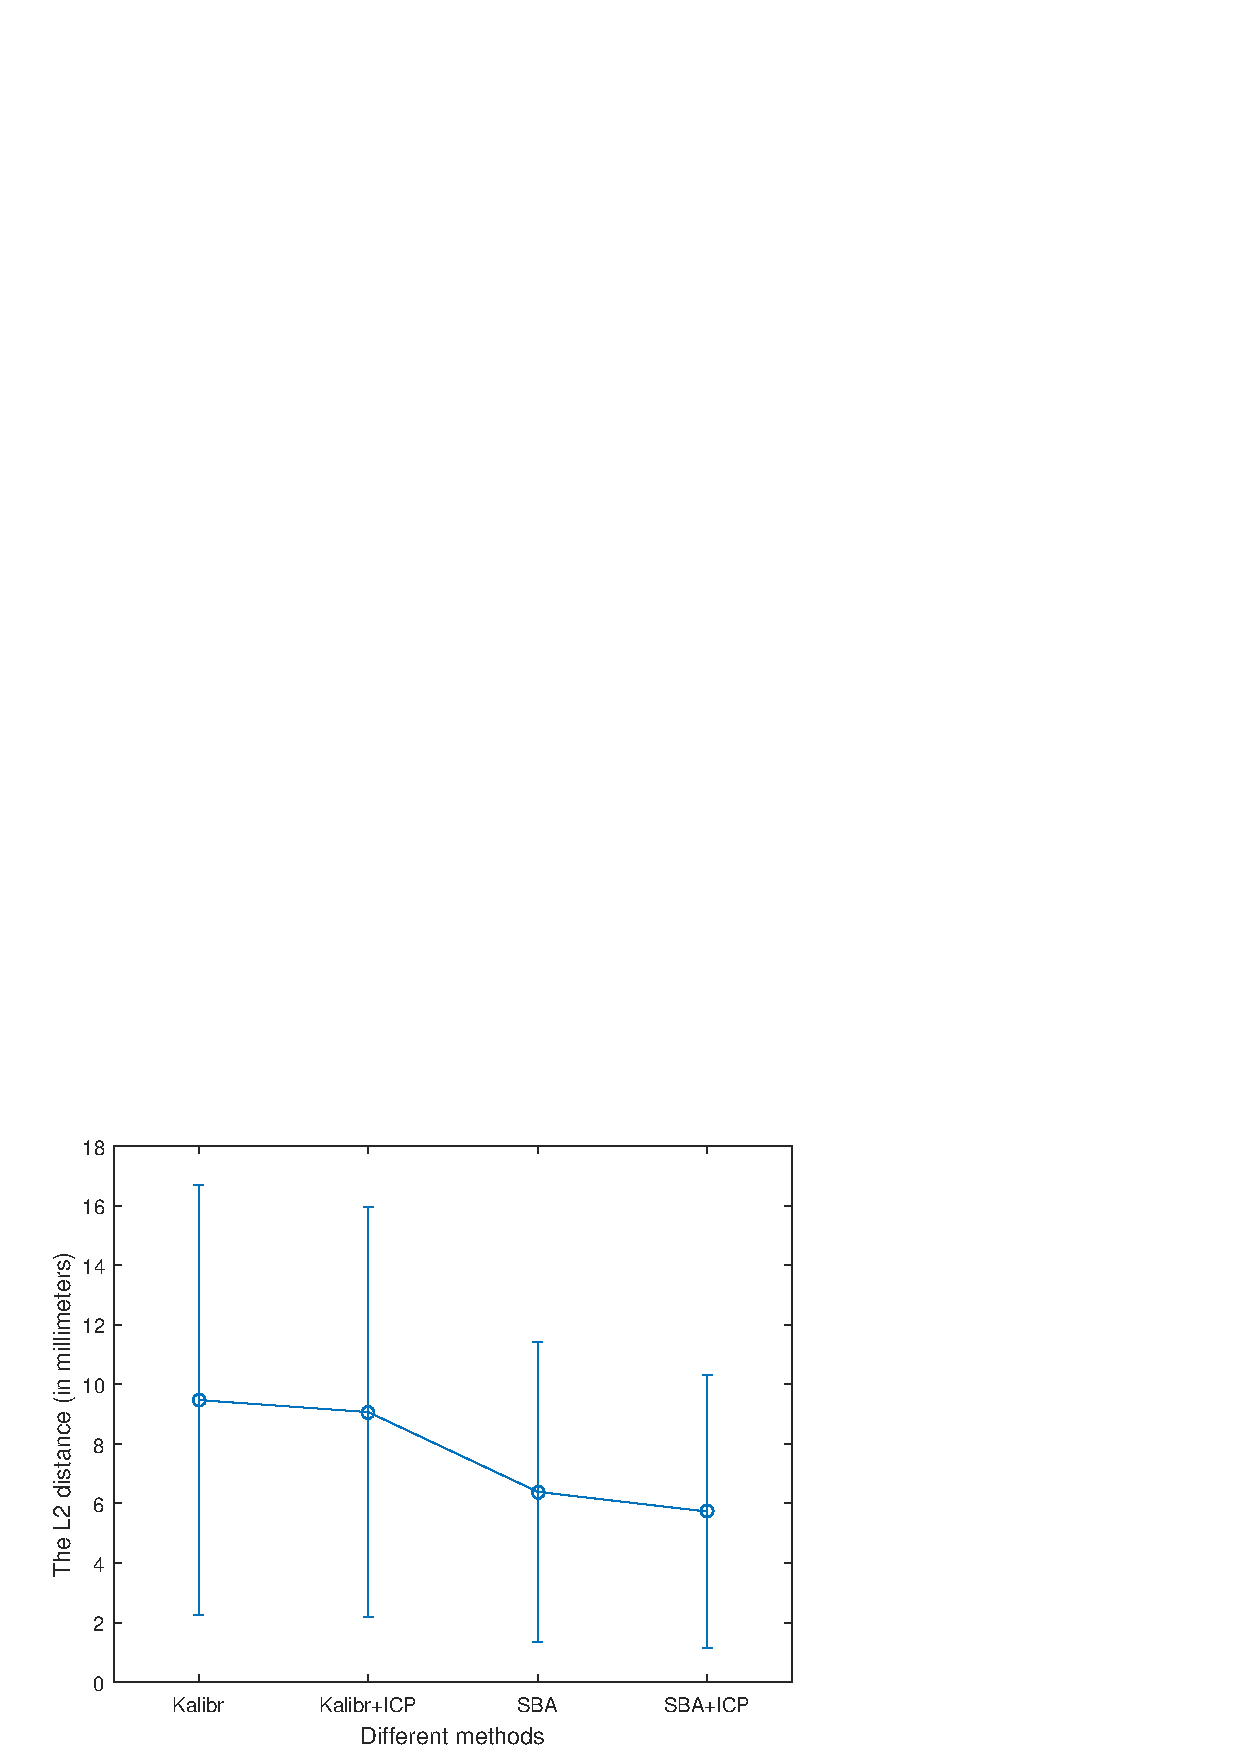
\includegraphics[width=\columnwidth]{image/errorbar.jpg}
	\caption{The error bars of the L2 distances of the point cloud reconstructed using different methods to the ground truth. \comments{(A) results by Kalibr~\cite{Maye2013Self}, (B) results by Kalibr~\cite{Maye2013Self} with our registration step, (C) results by our global calibration method, (D) results by our integrated method.} \xj{Use Kalibr, Kalibr+ICP, SBA, SBA+ICP in the figure to replace ABCD.}}
	\label{fig:errorbar}
\end{figure}
\comments{


\begin{figure}[ht]
%
\begin{minipage}[c]{0.49\linewidth}
  \centering
\includegraphics[width=4.4cm]{image/distribution.jpg}

  \centerline{(a)}\medskip
\end{minipage}
\hfill
\begin{minipage}[c]{0.49\linewidth}
  \centering
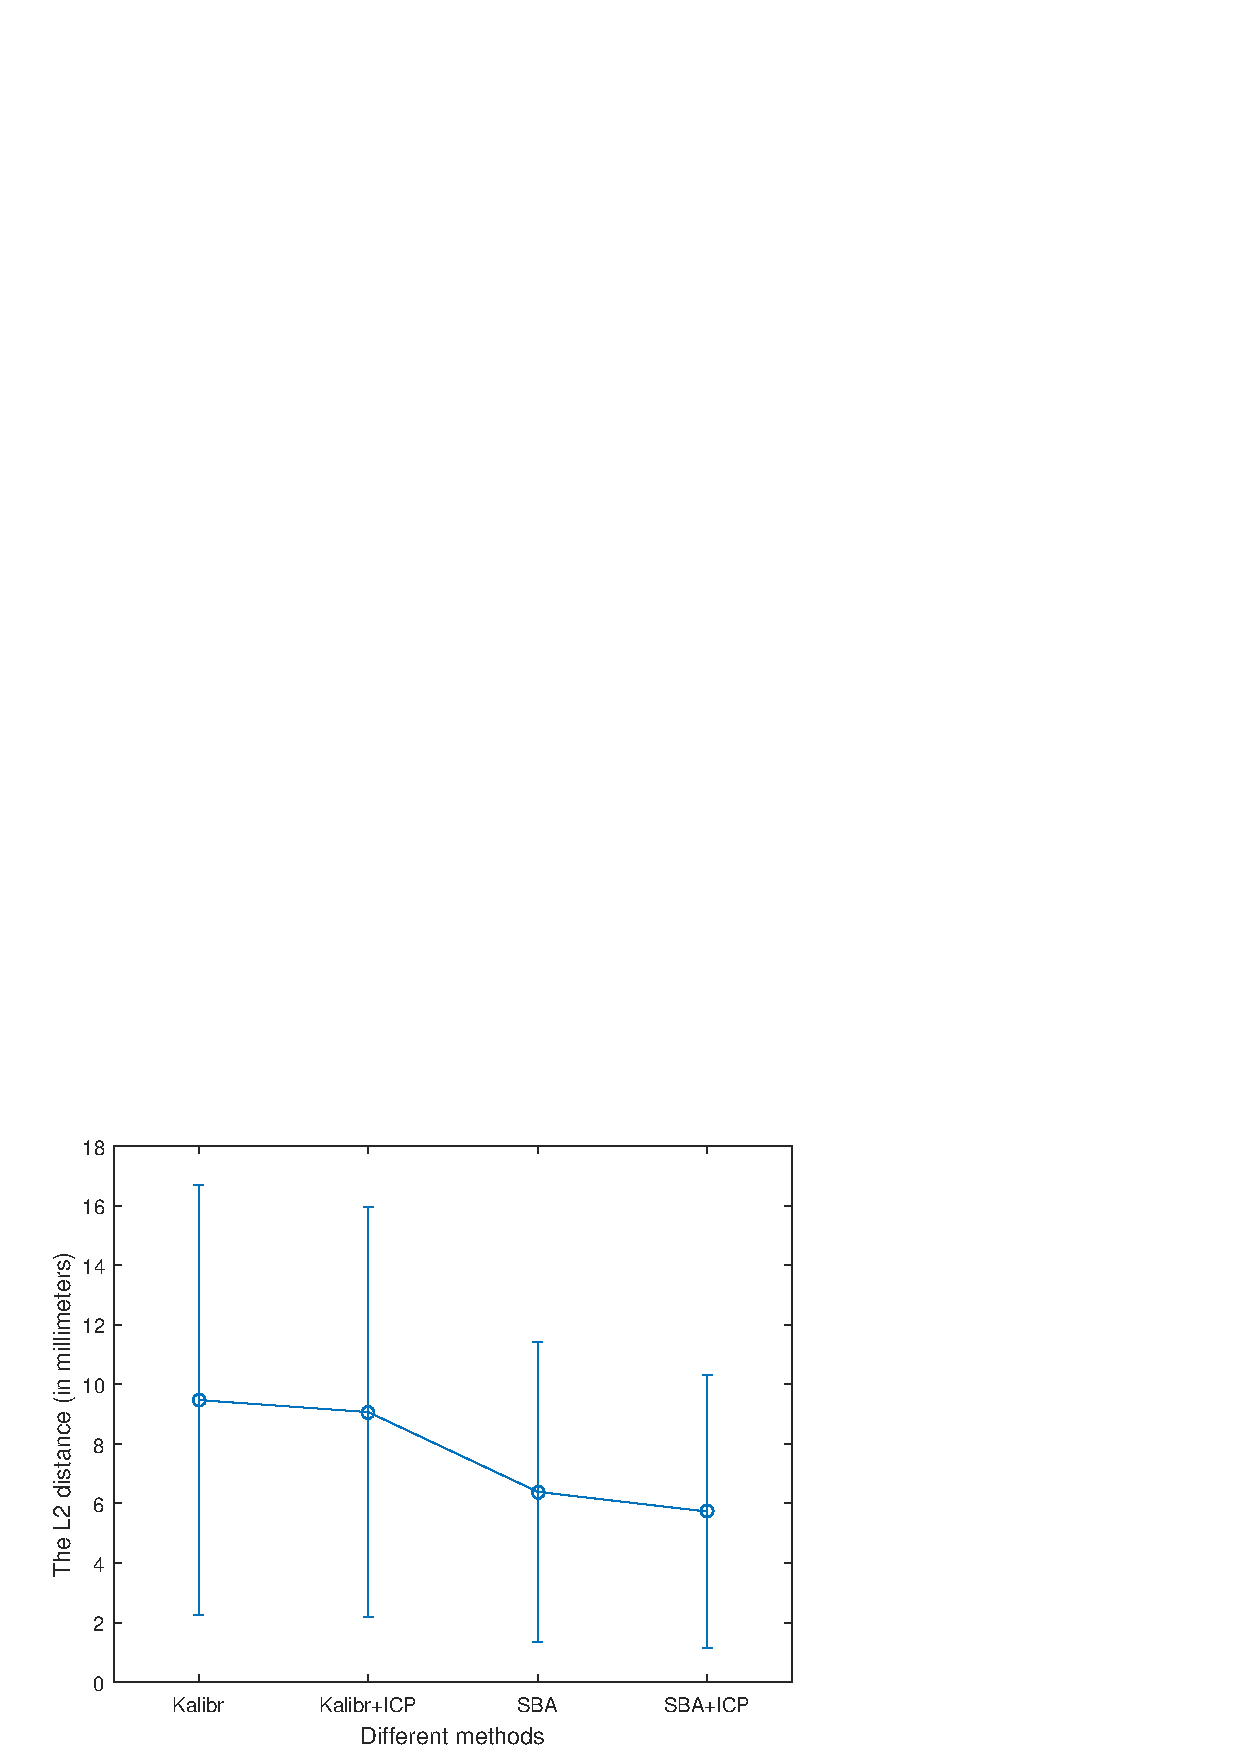
\includegraphics[width=4.4cm]{image/errorbar.jpg}

  \centerline{(b)}\medskip
\end{minipage}
%
\caption{The distribution and error bars of the L2 distances of the point cloud reconstructed using different methods to the ground truth. (A) results by Kalibr~\cite{Maye2013Self}, (B) results by Kalibr~\cite{Maye2013Self} with our registration step, (C) results by our global calibration method, (D) results by our integrated method.}
\label{fig:histogram}
\end{figure}
}

\noindent \textbf{More Reconstructed Models.}
%
We reconstruct the 3D point clouds of a human body standing in our multi-camera system using various methods.  We mark the point cloud in different views with different colors to show the quality of the fusion results. Fig.~\ref{fig:model_poses} shows the reconstruction results in different human pose which demonstrates our algorithm.\xj{demonstrates what of our algorithm?} 

The first row in Fig.~~\ref{fig:model_poses} shows the back side of a human body model using various methods. The point clouds in result (a) are distinctly separated from other views, as the pink and green views cover the whole surface of the model. Result (b) becomes a little better while the green view still covers the right side of the body. The point clouds align quite well in result (c) with small blemishes, the azure view is inside the model. (d) shows a well-aligned model. 
The second row in Fig.~~\ref{fig:model_poses} shows the left side of a human. The grey view in result (a) covers the surface and the black view is nearly inside the model especially on the shoulders and arms. Result (b) becomes a little better in black and grey view, however the green view covers the front of the model. There are similar problems in result (c), as the blue view covers the surface of the arm and head. Result (d) shows a well-aligned model, especially for the leg and arm with less separation between different views. 
The third row in Fig.~~\ref{fig:model_poses} shows the front of a human. The grey view covers the most surface of the right arm and the right chest, meanwhile the black view is inside the model in result (a). The point clouds align a little well in result (b), however the yellow view covers the left side of the body, and the blue view is nearly covered by other views. On the contrary, the blue view covers the right side of the body in result (c), especially on the arm and the shoulder. The point clouds more or less separated from other views in these results, while (d) shows a well-aligned model.
As we can see, the model reconstructed by our hybrid system has the highest quality.
\begin{figure}[ht]
	\centering
	\includegraphics[width=\columnwidth]{image/model.eps}
	\caption{The reconstruction results of a human body in different pose using four methods. (a) Kalibr~\cite{Maye2013Self}, (b) Kalibr+ICP, (c) SBA only, (d) SBA+ICP. We render the point clouds from different views with different colors.}
	\label{fig:model_poses}
\end{figure}


\comments{}

\section{conclusion}
We present an efficient system integrating a global multi-camera calibration with the 3D registered of point clouds. 
By a global bundle adjustment, we reduce the accumulative error and the inconsistence caused by the pairwise camera pose estimation, and achieve a set of accurate extrinsic parameters with less re-projection error. 
With the point cloud registration, the errors in depth estimation are balanced out and a high-quality 3D model is finally obtained. 
Our calibration algorithm has been tested on both re-projection error and ground truth data. The experimental results has proved that the two steps of our system are both necessary and effective, and more accurate models can be reconstructed using our method.







% References should be produced using the bibtex program from suitable
% BiBTeX files (here: strings, refs, manuals). The IEEEbib.bst bibliography
% style file from IEEE produces unsorted bibliography list.
% -------------------------------------------------------------------------
\bibliographystyle{IEEEbib}
\bibliography{icme2018template}

\end{document}
